\documentclass[10pt]{article}
\usepackage[utf8]{inputenc}
\usepackage[T1]{fontenc}
\usepackage{hyperref}
\hypersetup{colorlinks=true, linkcolor=blue, filecolor=magenta, urlcolor=cyan,}
\urlstyle{same}
\usepackage{amsmath}
\usepackage{amsfonts}
\usepackage{amssymb}
\usepackage[version=4]{mhchem}
\usepackage{stmaryrd}
\usepackage{caption}
\usepackage{multirow}
\usepackage{graphicx}
\usepackage[export]{adjustbox}
\graphicspath{ {./images/} }

\title{On Adaptive Extensions of Group Sequential Trials for Clinical Investigations}

\author{Qing Liu and Keaven M. Anderson}
\date{}

%New command to display footnote whose markers will always be hidden
\let\svthefootnote\thefootnote
\newcommand\blfootnotetext[1]{%
  \let\thefootnote\relax\footnote{#1}%
  \addtocounter{footnote}{-1}%
  \let\thefootnote\svthefootnote%
}

%Overriding the \footnotetext command to hide the marker if its value is `0`
\let\svfootnotetext\footnotetext
\renewcommand\footnotetext[2][?]{%
  \if\relax#1\relax%
    \ifnum\value{footnote}=0\blfootnotetext{#2}\else\svfootnotetext{#2}\fi%
  \else%
    \if?#1\ifnum\value{footnote}=0\blfootnotetext{#2}\else\svfootnotetext{#2}\fi%
    \else\svfootnotetext[#1]{#2}\fi%
  \fi
}

\begin{document}
\maketitle

In group sequential trials, it is important to obtain adequate data to assess overall benefits and risks of an experimental treatment for patients. To achieve this goal, we provide a general, formal framework for adaptively extending a group sequential trial to stop at any interim analysis time, often after a significance boundary for a clinical endpoint is crossed. For statistical inference. we propose to order the sample space by a class of well-ordered group sequential tests. On this basis, we develop a unified sequential statistical inference approach that is applicable to both interim monitoring and final analysis. We also show that the new ordering provides the foundation for the repeated confidence intervals procedure of Jennison and Turnbull.

KEY WORDS: Adaptive design; Group sequential design; Sample size adjustment; Sequential confidence interval; Sequential $p$ value.

\section*{1. INTRODUCTION}
Group sequential designs with asymmetrical boundaries are suitable for clinical trials to show beneficial effects of a new treatment versus control, while permitting early trial termination for lack of effectiveness or potential harm. However classical one-sided group sequential designs with formal futility boundaries (DeMets and Ware 1980, 1982) often are difficult to use in practice. First, a futility boundary must be strictly enforced to maintain control of the type I error rate. Second, the group sequential test does not incorporate any additional data obtained after a significance or futility boundary is crossed.

In actuality, the stopping boundaries for a clinical trial are considered guidelines. Other relevant secondary efficacy and safety data, as well as external information, also are taken into account in making a decision to stop the trial early (DeMets 1984; Lan and Wittes 1994; Whitehead 1999; Lan, Lachin, and Bautista 2003). In fact, it is now standard practice to provide a Data Safety and Monitoring Board (DSMB) with a comprehensive list of trial-related summaries (see tables 5.1 and 5.2 of Ellenberg, Fleming, and DeMets 2002, pp. 73-74). Canner (1983) eloquently stated that "decision-making in clinical trials is complicated and often protracted... no single statistical decision rule or procedure can take the place of well-reasoned consideration of all aspects of the data by a group of concerned, competent and experienced persons with a wide range of scientific backgrounds and points of view."

Various secondary efficacy and safety data are required for interim decisions, because the primary endpoint alone often is not sufficient to address all scientific and clinical objectives while balancing ethical considerations. The U.S. Code of Federal Regulations (21 CFR 312.21) clearly states that "Phase 3 studies... are intended to gather the additional information about effectiveness and safety that is needed to evaluate the overall benefit-risk relationship of the drug...." Ultimately, it is a favorable benefit-risk profile of the medical product for patients that will lead to its marketing approval and positive public health impact. It is not unusual for a DSMB to recommend extending a trial to collect more data on secondary or safety endpoints, even though the significance boundary for the primary endpoint already has been crossed. An excellent example is the

\footnotetext{Qing Liu is Senior Research Fellow, Statistical Science, J\&J Pharmaceutical Research and Development, L.L.C., Raritan, NJ 08869 (E-mail: \href{mailto:qliu2@its.jnj.com}{qliu2@its.jnj.com}). Keaven M. Anderson is Executive Director, Late-Stage Statistics, Merck Research Laboratories, North Wales, PA 19454. The authors are indebted to two referees, an associate editor, and the editor for their constructive comments and suggestions, which have greatly enhanced the content and presentation of this article.
}
fluconazole trial described by Ellenberg et al. (2002, pp. 36-37). Next we present the motivating example.

Example. Nosocomial pneumonia (NP) is the second most common nosocomial infection after urinary tract infection and is the most common infection in the intensive care unit setting. Overall, NP accounts for 15-18\% of all hospital-acquired infections and is the leading cause of death from nosocomial infection. The mortality rate for NP exceeds 30\%. The clinical cure rate is around 50\% with existing options of various antibiotics.

Now consider a clinical trial to evaluate whether a new regimen can improve the clinical cure rate over an existing regimen. It also is important to evaluate mortality and to quantify other changes in morbidity. A group sequential design is a suitable option, because the primary endpoint (i.e., clinical cure) is readily evaluated over 14 days, and the enrollment is not very rapid. An important feature is that the trial may be continued to allow evaluation of a 30-day mortality endpoint even though a significance boundary for the primary endpoint has been crossed. It also is expected that a more aggressive combination regimen may increase the risk for serious adverse reactions. Thus close safety monitoring is required, and the trial may be extended to clarify emerging safety patterns.

This example represents the general problem that a group sequential trial may need to be extended for secondary efficacy or safety reasons, even when the significance boundary for the primary endpoint is crossed. There also are natural reasons for additional data (Whitehead 1992). For many group sequential trials, the clinical endpoint is not quickly observed. Although patients who are already enrolled in the trial are being followed for the clinical endpoint, new patients who meet the trial entry criteria are continuously enrolled without having to wait for the interim results. Thus additional data exist, which almost always are collected after a stopping boundary is crossed. For many applications, clinical events recorded by the investigators must be evaluated independently by an adjudication committee. Additional adjudicated events will be observed after an interim analysis due simply to delays introduced by the adjudication process.

The ICH-E9 guideline (ICH 1998) and the intent-to-treat (ITT) principle require that statistical analyses include all randomized patients. A recent CHMP guidance for adaptive designs (CHMP 2007) also recommends that final analyses, including estimates and confidence intervals, be based on the ITT

\footnotetext{© 2008 American Statistical Association\\
Journal of the American Statistical Association\\
December 2008, Vol. 103, No. 484, Theory and Methods\\
DOI 10.1198/016214508000000986
}
population. For group sequential trials, there are several proposals for handling additional data (Whitehead 1992; Hall and Liu 2002; Hall and Ding 2008). These proposals are concerned only with inference at the final analysis and do not allow sequential monitoring and inference for an ongoing trial.

Following the ideas of Liu and Pledger (2006) for a two-stage design, in Section 2 we propose a new approach for ordering the sample space by a class of well-ordered group sequential tests indexed by a parameter $\mu$ in (0, 1). This ordering yields sequential $p$ values and confidence intervals that are consistent with the sequential testing procedure and use all existing data. In Section 3 we provide a general framework that allows extension of group sequential trials with or without sample size adjustment. For designs with options for sample size adjustment, we provide corresponding methods for obtaining sequential $p$ values and confidence intervals. We then develop a method for obtaining unbiased estimates for a parameter, following a variance-spending approach of Fisher (1998), for which unequal weights are used. In Section 4 we provide numerical illustrations, including simulation results, of the design for the motivating example. We provide proofs of the theorems in a supplemental article (Liu and Anderson 2008), available at http:// \href{http://www.amstat.org/publications/jasa/supplemental_materials}{www.amstat.org/publications/jasa/supplemental\_materials}. We show there that the extended group sequential designs cover a wide area of practical applications. In particular, we demonstrate that standard methods for testing multiple hypotheses can be easily implemented with the proposed sequential $p$ values. We also give details of examples documenting difficulties with the inferential procedures summarized in Jennison and Turnbull (2000, p. 180).

\section*{2. INFERENCE FOR GROUP SEQUENTIAL DESIGNS}
\subsection*{2.1 Test Procedure}
For a clinical endpoint, let $\Delta$ be the effect size of a new treatment compared with a control, where, without loss of generality, a positive $\Delta$ implies superior efficacy. We want to perform a group sequential test against the null hypothesis $H: \Delta \leq 0$ in favor of the alternative hypothesis $A: \Delta>0$ at $K$ specified sequential analysis times. For clinical development, a new treatment often fails the superiority promise; therefore, we would like to stop the trial early through futility tests to rule out an effect size that is substantially less than a minimal effect size, $\delta_{\text {min }}$, of interest.

For $k=1,2, \ldots, K$, let $Z_{k}$ be the test statistic against the null hypothesis $H$ in favor of the alternative hypothesis $A$. For a given significance level $\alpha$ (e.g., $\alpha=.025$ for trials intended for regulatory submissions), we calculate the significance boundary values, $b_{k}$, for $k=1,2, \ldots, K$ such that


\begin{equation*}
P_{\Delta=0}\left\{Z_{1} \geq b_{1} \cup Z_{2} \geq b_{2} \cup \cdots \cup Z_{K} \geq b_{K}\right\}=\alpha . \tag{1}
\end{equation*}


Let $\beta$ be a type II error rate for not being able to reject the null hypothesis by the group sequential test, $Z_{k} \geq b_{k}$, for at least one $k=1,2, \ldots, K$. We calculate nonbinding futility boundary values, $a_{k}$, satisfying $a_{k}<b_{k}$, for $k=1,2, \ldots, K-1$ and $a_{K}=$ $b_{K}$, such that


\begin{align*}
& P_{\Delta=\delta_{\min }}\left\{Z_{1}<a_{1}\right\}+P_{\Delta=\delta_{\min }}\left\{a_{1} \leq Z_{1}<b_{1}, Z_{2}<a_{2}\right\}+\cdots \\
& +P_{\Delta=\delta_{\min }}\left\{a_{1} \leq Z_{1}<b_{2}, \ldots\right. \\
& \left.\quad a_{K-1} \leq Z_{K-1}<b_{K-1}, Z_{K}<a_{K}\right\}=\beta \tag{2}
\end{align*}


A futility boundary such as that given in (2) often is referred to as a nonbinding boundary. It is now implemented as the default procedure in the East software, version 5.2, because of practical demands and the Food and Drug Administration's reluctance to accept a traditional binding futility boundary. There are other nonbinding approaches to interim monitoring for futility, including the use of conditional or predictive power, or posterior probabilities. These various methods do not change the inference proposed in this article. For simplicity, we use only nonbinding boundaries given in (2) herein.

With any significance boundary following (1), the type I error rate for rejecting the null hypothesis $H$ would be exactly $\alpha$ if the trial would never be terminated for futility. If both the significance and futility boundaries satisfying (1) and (2) are strictly followed (i.e., the trial must stop if a boundary is crossed), then the type I error rate for rejecting the null hypothesis $H$ is less than $\alpha$. An advantage of calculating separate significance and futility boundaries according to (1) and (2) is that it provides the flexibility to continue the trial even if the futility boundary is crossed (Proschan, Lan, and Wittes 2006, p. 91). Such flexibility often is desirable when a lack of efficacy early in a trial is due to underlying issues of compliance and inexperience that can be resolved later as the trial proceeds. For most applications, it is important to quantify all of the benefits and risks of a new treatment. When the significance boundary for a primary endpoint is crossed, data for secondary efficacy or safety endpoints may not be sufficient. Thus another desirable design feature is to allow the trial to continue beyond the interim analysis when the significance boundary is crossed. We show that this is possible if a significance boundary is calculated according to (1).

When neither the futility nor the significance boundary is followed strictly, the stopping time $\tau$, taking values $1,2, \ldots, K$, depends on the totality of the accumulating data, not just on the test statistic in question. Therefore, $\tau$ may precede, coincide with, or exceed the boundary crossing time. For simplicity, a group sequential design with any stopping time $\tau$ is referred to as an extended group sequential design (EGS design). Accordingly, an extended group sequential test (EGS test) refers to a test for checking whether $Z_{k} \geq b_{k}$ for $k=1,2, \ldots, \tau$ for any stopping time $\tau$ taking values in $\{1,2, \ldots, K\}$. In notation, an EGS test is positive if the event $\bigcup_{k=1}^{K}\left[\{\tau=k\} \cap \bigcup_{i=1}^{k}\left\{Z_{i} \geq\right.\right.$ $\left.\left.b_{i}\right\}\right]$ occurs. We point out that an EGS test applies only to a single null hypothesis, whereas an EGS design can have multiple EGS tests that are subject to a common stopping time, $\tau$. The following theorem establishes the validity of an EGS test.

Theorem 1. Assume that $b_{1}, b_{2}, \ldots, b_{K}$ are chosen to satisfy (1) for a given $\alpha \in(0,1)$. Then


\begin{equation*}
P_{\Delta=0}\left\{\bigcup_{k=1}^{K}\left[\{\tau=k\} \cap \bigcup_{i=1}^{k}\left\{Z_{i} \geq b_{i}\right\}\right]\right\} \leq \alpha \tag{3}
\end{equation*}


for any stopping rule $\tau$ with a range in $\{1,2, \ldots, K\}$.\\
The proof for the theorem is straightforward and is given in the supplemental article. Intuitively, the rejection event, $\bigcup_{k=1}^{K}\left[\{\tau=k\} \cap \bigcup_{i=1}^{k}\left\{Z_{i} \geq b_{i}\right\}\right]$, often is loosely written as $Z_{1} \geq b_{1} \cup \cdots \cup Z_{\tau} \geq b_{\tau}$, making it obvious that the procedure\\
controls the type I error rate. Despite its mathematical simplicity, the theorem is fundamental to all of the inferential procedures developed in the article. For a classical group sequential design, the stopping time, denoted by $\tau_{0}$, depends only on the test statistics $Z_{k}$ for $k=1,2, \ldots, K$. Specifically, $\tau_{0}=k$ if and only if $k$ is the time at which either the significance or (binding) futility boundary is first crossed, which is a necessary restriction to control the type I error rate (Lan et al. 2003). In contrast, $\tau$ in Theorem 1 can be any stopping time. The profound implication is that the decision to continue or stop the trial now can be based on a review of the totality of the accumulating data. A procedure with the same property has been given by Jennison and Turnbull (1989), through which the null hypothesis is rejected if and only if a repeated lower confidence bound exceeds 0.

\subsection*{2.2 Principles of Group Sequential Inference}
For group sequential trials, statistical inference is important while the trial is ongoing and when the trial is stopped. We propose three basic principles for group sequential inference, which form the foundation for interpreting trial results. We start with an ordering of the sample space and define an overall $p$ value as the null probability of more extreme observations. We assume that this ordering will be used in probabilistic evaluations of a group sequential inference procedure according to the strong repeated sampling principle (Cox and Hinkley 1974, p. 45).

Basic Principles.

\begin{itemize}
  \item[I.] An ordering is defined on the sample space consisting of all sample paths $\left\{\tau ; Z_{1}, Z_{2}, \ldots, Z_{\tau}\right\}$, where $\tau$ is a stopping time determined by the totality of the accumulating data.
  \item[II.] A null hypothesis is rejected by a group sequential test if and only if its significance boundary is crossed at or before $\tau$, or the overall $p$ value, denoted by $p_{\tau}$, is less than or equal to the significance level $\alpha$.
  \item[III.] For any $\mu \in(0,1)$, the group sequential test corresponding to $p_{\tau} \leq \mu$ is consistent with the underlying ordering of the sample space.
\end{itemize}

Principle I is introduced to permit sequential monitoring and inference for an extended group sequential trial with a flexible stopping time $\tau$. Principle II is an extension of property (i) of Jennison and Turnbull (2000, pp. 180-181) for a classical group sequential test, by which a trial stops when a boundary is first crossed. Principle III is introduced to maintain monitoring and inferential consistency at different significance levels.

Hacking (1965, p. 1) stated that "the problem of the foundation of statistics is to state a set of principles which entail the validity of all correct statistical inference, and which do not imply that any fallacious inference is valid." For group sequential trials, the three basic principles are necessary for evaluating probabilistic properties of $p$ values in hypothetical replications following the strong repeated-sampling principle. From this frequentist's perspective, a probabilistic evaluation of a statistical procedure should take into account not only what has happened for the current trial, but also what would have happened had the trial been replicated. From practical experience, various deviations from the original group sequential design can occur, including a flexible stopping time, a change in sample size, a change in significance level, and changes in the number or timing of interim analyses. For this article, the immediate benefit of stating the three basic principles is to guide the development of a unified sequential inference approach, applicable to both monitoring and final analysis, such that the resulting inference is robust against the various practical deviations just mentioned. In the supplemental article, the three basic principles also are used to evaluate other group sequential procedures and their consequences for monitoring and inference.

\subsection*{2.3 Ordering of the Sample Space}
Coherent sequential monitoring and inference concerning the underlying parameter can be developed if the sample space can be properly ordered and the $p$ values are calculated carefully. Motivated by the work of Liu and Pledger (2006), we extend an EGS test for the given significance level $\alpha$, say, $\alpha=.025$, to a class of EGS tests indexed by a parameter $\mu \in(0,1)$. We assume that for any $\mu \in(0,1)$ there exist $b_{k}(\mu)$ for $k=$ $1,2, \ldots, K$, such that


\begin{equation*}
P_{\Delta=0}\left\{Z_{1} \geq b_{1}(\mu) \cup Z_{2} \geq b_{2}(\mu) \cup \cdots \cup Z_{K} \geq b_{K}(\mu)\right\}=\mu . \tag{4}
\end{equation*}


This creates a class of boundaries indexed by $\mu \in(0,1)$. We define the class as well ordered if the boundary $b_{k}(\mu)$ is continuous and decreasing in $\mu$ and converges to $\infty$ as $\mu \rightarrow 0$ for any $k=1,2, \ldots, K$.

A class of well-ordered significance boundaries defines an ordering of the sample space for the endpoint in question, which consists of sample paths of the form $\underline{\omega}=\left\{\tau ; Z_{1}, Z_{2}, \ldots, Z_{\tau}\right\}$, where $\tau$ is any stopping time based on the totality of the accumulating data. For any such sample path, there exist $\hat{\mu}^{(k)}=$ $\sup \left\{\mu: Z_{k} \leq b_{k}(\mu)\right\}$ for $k=1,2, \ldots, \tau$. Let


\begin{equation*}
p_{\tau}=\min \left\{\hat{\mu}^{(k)}: k=1,2, \ldots, \tau\right\} . \tag{5}
\end{equation*}


Then $Z_{k} \leq b_{k}\left(p_{\tau}\right)$ for all $k=1,2, \ldots, \tau$, and $Z_{k}=b_{k}\left(p_{\tau}\right)$ for at least one $k$ in $1,2, \ldots, \tau$. Two sample paths, $\underline{\omega}^{\prime}$ and $\underline{\omega}^{\prime \prime}$, are said to follow the order $\preceq$ if and only if their corresponding minimum $\mu$ values, $p_{\tau^{\prime}}^{\prime}$ and $p_{\tau^{\prime \prime}}^{\prime \prime}$, follow the natural order $p_{\tau^{\prime}}^{\prime} \geq p_{\tau^{\prime \prime}}^{\prime \prime}$ for real numbers. Apparently, if $\underline{\omega}^{\prime} \preceq \underline{\omega}^{\prime \prime}$ and $\underline{\omega}^{\prime \prime} \leq \underline{\omega}^{\prime \prime \prime}$, then $\underline{\omega}^{\prime} \leq \underline{\omega}^{\prime \prime \prime}$. Thus the ordering is well defined.

In the supplemental article we compare the proposed ordering with those in the literature and illustrate their consequences on resulting $p$ values. Note that the ordering is still defined when the boundary values are calculated according to the $\alpha$ spending approach of Lan and DeMets (1983), where the number or timing of interim analyses may not be specified in advance. This may not be true when other methods for calculating boundaries are used, however.

\subsection*{2.4 Sequential and Final $p$ Values}
We define $p$ values for the proposed ordering with a class of well-ordered boundaries. For any $\mu \in(0,1)$, let $\mu_{k}=$ $P_{\Delta=0}\left[\bigcup_{i=1}^{k}\left\{Z_{i} \geq b_{i}(\mu)\right\}\right]$ for $k=1,2, \ldots, K$. The $\mu$-level full group sequential test (FGS test), $\bigcup_{i=1}^{K}\left\{Z_{i} \geq b_{i}(\mu)\right\}$, induces a $\mu_{k}$-level FGS test, $\bigcup_{i=1}^{k}\left\{Z_{i} \geq b_{i}(\mu)\right\}$, for $k=1,2, \ldots, K$. Thus (4) in Section 2.3 induces sequentially $K$ classes of FGS tests. The class of boundaries for each of the induced classes is\\
obviously well-ordered for $\mu \in(0,1)$. For the induced class at the $k$ th interim analysis, define


\begin{equation*}
p_{k}=\sup \left[\mu: \max _{1 \leq i \leq k}\left\{Z_{i}-b_{i}(\mu)\right\} \leq 0\right] . \tag{6}
\end{equation*}


We call $p_{1}, p_{2}, \ldots, p_{K}$ sequential $p$ values. For any stopping time $\tau$, the final $p$ value is $p_{\tau}=\sum_{k=1}^{K} p_{k} I_{\tau=k}$, where $I_{\tau=k}$ is the indicator function for the event $\{\tau=k\}$. It is easily shown that this definition of the final $p$ value is identical to the minimum $\mu$ value given by (5). The sequential and final $p$ values have the properties outlined in the following theorem.

Theorem 2.

\begin{itemize}
  \item[a.] $p_{k} \leq \mu$ is equivalent to $\bigcup_{i=1}^{k}\left\{Z_{i} \geq b_{i}(\mu)\right\}$ for any $\mu \in$ $(0,1)$ and $k=1,2, \ldots, K$.
  \item[b.] $P_{\Delta=0}\left\{p_{k} \leq \mu\right\} \leq \mu_{k} \leq \mu$ for any $\mu \in(0,1)$ and $k=$ $1,2, \ldots, K$.
  \item[c.] $p_{1} \geq p_{2} \geq \cdots \geq p_{K}$.
  \item[d.] $p_{\tau} \leq \mu$ is equivalent to $\bigcup_{k=1}^{K}\left[\{\tau=k\} \cap \bigcup_{i=1}^{k}\left\{Z_{i} \geq\right.\right.$ $\left.\left.b_{i}(\mu)\right\}\right]$ for any $\mu \in(0,1)$.
  \item[e.] $P_{\Delta=0}\left\{p_{\tau} \leq \mu\right\} \leq \mu$ for any $\mu \in(0,1)$.
  \item[f.] Let $p_{\tau}^{\prime} \leq \mu$ be equivalent to $\bigcup_{k=1}^{K}\left[\{\tau=k\} \cap \bigcup_{i=1}^{k}\left\{Z_{i} \geq\right.\right.$ $\left.\left.b_{i}(\mu)\right\}\right]$ for any $\mu \in(0,1)$. Then $p_{\tau}^{\prime}=p_{\tau}$ with probability 1 .
\end{itemize}

For the proposed ordering, the theorem establishes a unified approach to $p$ values for assessing the smallest type I error rates for rejecting the null hypothesis. By construction, the sequential $p$ values follow the three basic principles of group sequential inference. As a result, the sequential $p$ values have several features: (a) The final $p$ value, $p_{\tau}$, adheres to the ITT principle that all available data are analyzed; (b) sample paths reaching the same boundary have identical $p$ values; and (c) $p_{\tau}$ is always significant if the significance boundary is crossed at any stage, not requiring $Z_{\tau} \geq b_{\tau}$. In the discussion in Section 5, we elaborate on how these $p$ values are to be interpreted and also point out their limitations.

\subsection*{2.5 Sequential and Final Confidence Intervals}
The procedure outlined in Section 2.1 can be generalized to test against the null hypothesis $H_{\delta}: \Delta \leq \delta$ in favor of the alternative hypothesis $A_{\delta}: \Delta>\delta$. Following Jennison and Turnbull (2000, p. 191), let $Z_{k}(\delta)=Z_{k}-\delta \mathcal{I}_{k}^{1 / 2}$ for $k=1,2 \ldots, K$, where $\mathcal{I}_{k}$ for $k=1,2, \ldots, K$ are observed information levels. Then, for many test statistics that are asymptotically normally distributed, the equation


\begin{equation*}
P_{\Delta=\delta}\left\{Z_{1}(\delta) \geq b_{1} \cup Z_{2}(\delta) \geq b_{2} \cup \cdots \cup Z_{k}(\delta) \geq b_{k}\right\}=\alpha_{k} \tag{7}
\end{equation*}


holds approximately for $\alpha_{k}=P_{\Delta=0}\left\{Z_{1} \geq b_{1} \cup Z_{2} \geq b_{2} \cup \cdots \cup\right.$ $\left.Z_{k} \geq b_{k}\right\}$, for which the boundary values $b_{1}, b_{2}, \ldots, b_{k}$ are calculated to satisfy (1). For any $k$, the largest $\delta$ such that $H_{\delta}$ is rejected in favor of $A_{\delta}$ at or before the $k$ th interim analysis is given by


\begin{equation*}
\hat{\Delta}_{k}^{L}=\max _{1 \leq i \leq k}\left\{\left(Z_{i}-b_{i}\right) / \mathcal{I}_{i}^{1 / 2}\right\} . \tag{8}
\end{equation*}


We call $\hat{\Delta}_{k}^{L}$ for $k=1,2, \ldots, K$ sequential lower confidence bounds. Their properties are summarized in the following theorem.

Theorem 3. Let eq. (7) be true for any $\delta \in(-\infty, \infty)$ and $k=1,2, \ldots, K$. Then the following properties hold:

\begin{itemize}
  \item[a.] $\hat{\Delta}_{k}^{L} \geq 0$ is equivalent to $\bigcup_{i=1}^{k}\left\{Z_{i} \geq b_{i}\right\}$ for $k=1,2$, $\ldots, K$.
  \item[b.] $P_{\Delta}\left\{\hat{\Delta}_{k}^{L}<\Delta\right\}=1-\alpha_{k}$ for $k=1,2, \ldots, K$.
  \item[c.] $\hat{\Delta}_{1}^{L} \leq \hat{\Delta}_{2}^{L} \leq \cdots \leq \hat{\Delta}_{K}^{L}$.
  \item[d.] $P_{\Delta}\left\{\hat{\Delta}_{\tau}^{L}<\Delta\right\} \geq 1-\alpha$ and $P_{\Delta=0}\left\{\hat{\Delta}_{\tau}^{L} \geq 0\right\} \leq \alpha$ are true for any stopping time $\tau$.
\end{itemize}

More generally, the $(1-\mu)$-level sequential lower confidence bounds for any $\mu \in(0,1 / 2]$ are given by $\hat{\Delta}_{k}^{L}(\mu)=$ $\max _{1 \leq i \leq k}\left[\left\{Z_{i}-b_{i}(\mu)\right\} / \mathcal{I}_{i}^{1 / 2}\right]$ for $k=1,2, \ldots, K$, to which the results in Theorem 3 also are applicable. In particular, by part a of both Theorems 2 and 3, we know that for any $\mu \in(0,1 / 2]$, the sequential lower confidence bounds can be obtained by inverting tests by the sequential $p$ values at the significance level $\mu$. Because the sequential lower confidence bounds are cumulative maxima of the repeated lower confidence bounds, which are constructed for the test problem in Section 2.1 according to the approach of Jennison and Turnbull (1989), an important revelation is that the repeated lower confidence bounds are fundamentally dependent on the ordering of the sample space by a class of well-ordered group sequential tests described in Section 2.3. Another revelation is that repeated lower confidence bounds lead to a final lower confidence bound, which is the sequential lower confidence bound at trial termination.

It is customary to provide confidence intervals for a parameter of interest. Because the sequential lower confidence bounds have been given earlier, we only have to provide sequential upper confidence bounds. Consistent with the two-one-sided tests procedure of Proschan (1999), the sequential upper confidence bounds can be constructed similarly by inverting the sequential test against the null hypothesis $\Delta \geq \delta$ in favor of the alternative hypothesis $\Delta<\delta$ at the one-sided significance level $\alpha$. The sequential upper confidence bounds are given by $\hat{\Delta}_{k}^{U}=\min _{1 \leq i \leq k}\left\{\left(Z_{i}+b_{i}\right) / \mathcal{I}_{i}^{1 / 2}\right\}$ for $k=1,2, \ldots, K$. Note that ( $\hat{\Delta}_{k}^{L}, \hat{\Delta}_{k}^{U}$ ) for $k \geq 1$ are intersections of the repeated confidence intervals of Jennison and Turnbull (1989). To emphasize the intervals' sequential inferential nature, we formally refer to them as sequential confidence intervals. It is easily shown that for any stopping time $\tau$, the final confidence interval $\left(\hat{\Delta}_{\tau}^{L}, \hat{\Delta}_{\tau}^{U}\right)$ has a probability of coverage at least $(1-2 \alpha)$, assuming that the effect size of the treatment is homogeneous over time. When the effect size is heterogeneous, the coverage probability is undefined.

The sequential confidence interval procedure also leads to a point estimation procedure. For $\mu=.5$, let the resulting sequential confidence bounds be denoted by, say, $\hat{\Delta}_{k}^{L}(.5)$ and $\hat{\Delta}_{k}^{U}(.5)$ for $k=1,2, \ldots, K$. Then, for a given $k$, any value between $\hat{\Delta}_{k}^{L}(.5)$ and $\hat{\Delta}_{k}^{U}(.5)$ is a median unbiased estimator of $\Delta$. In particular, we propose using the sequential median unbiased estimators $\hat{\Delta}_{k}^{\text {Med }}=\left\{\hat{\Delta}_{k}^{L}(.5)+\hat{\Delta}_{k}^{U}(.5)\right\} / 2$ for $k=1,2, \ldots, K$. At the stopping time $\tau$, the final median unbiased estimator is $\hat{\Delta}_{\tau}^{\text {Med }}$. Finally, in the supplemental article we derive the sequential upper futility bounds, given by


\begin{equation*}
\hat{\Delta}_{k}^{F U}=\min _{1 \leq i \leq k}\left[\left\{Z_{i}+\left(\mathcal{I}_{i}^{1 / 2} \delta_{\min }-a_{i}\right)\right\} / \mathcal{I}_{i}^{1 / 2}\right] \tag{9}
\end{equation*}


for $k=1,2, \ldots, K$, by which $\hat{\Delta}_{k}^{F U}<\delta_{\text {min }}$ at the $k$ th interim analysis is equivalent to $Z_{i}<a_{i}$ for some $i=1,2, \ldots, k$.

To monitor an ongoing trial, it is convenient to plot the sequential lower and upper confidence bounds $\hat{\Delta}_{i}^{L}$ and $\hat{\Delta}_{i}^{U}$, median unbiased estimates $\hat{\Delta}_{i}^{\text {Med }}$, and upper futility bounds $\hat{\Delta}_{i}^{F U}$ against information levels $\mathcal{I}_{i}$ for $i=1,2, \ldots, k$, where $k=$ $1,2, \ldots, K$. This plot is useful for checking whether boundaries have been crossed. It also provides visual clues on treatment effect over time. An example of such a plot is given in Section 4.2.

\section*{3. ADAPTIVE TRIAL EXTENSIONS}
\subsection*{3.1 A General Framework}
We assume that the trial has $K$ stages and $K$ analyses. To assess the overall benefits and risks, we propose an adaptive extension of the trial to stop at a future interim analysis after a significance boundary is crossed. We also allow sample size adaptation when the planned total sample size is not adequate. For applications with short treatment and follow-up, the planned sample size for the $k$ th stage is $n_{k}$ for $k=1,2, \ldots, K$. The $k$ th-stage data refer to the totality of data from patients who are enrolled in the $k$ th stage. The $k$ th-stage accumulating data refer to the totality of data from patients who are enrolled in the first $k$ stages of the trial.

We define a sequence of adaptation rules for $k=1,2, \ldots$, $K-1$. For the $k$ th interim analysis, the adaptation rules consist of a triplet $\left\langle d_{k}, t_{k}, g_{k}\right\rangle$. The termination decision rule, $d_{k}$, is a binary variable, taking a value of 1 or 0, where $d_{k}=1$ represents the event that the decision is reached to terminate the trial at a single adaptively chosen future time, $t_{k}=k+$ $1, \ldots, K$, and $d_{k}=0$ represents the event that the decision has not been reached to terminate the trial at a future time, for which case $t_{k}=K$ is the default value. The sample size rule, $g_{k}$, adaptively chooses the numbers of patients, $\hat{m}_{j k}$, for $j=k+1, \ldots, K$ of the remaining $K-k$ stages to meet specific sample size criteria. The sequence of termination decision rules, $d_{k}$, for $k=1,2, \ldots, K-1$ defines a termination decision time, $\tau^{*}=\inf \left\{k: d_{k}=1,1 \leq k \leq K-1\right\}$, and, together with the sequence $t_{k}$ for $1 \leq k \leq K-1$, defines the stopping time $\tau=t_{\tau^{*}}$.

Typically, one would choose $d_{k}=1$ if the significance boundary for the primary endpoint is already or nearly crossed, and the focus is shifted to other aspects of the trial. Alternatively, one also could choose $d_{k}=1$ at a certain major interim analysis when all of the assumptions are reevaluated and the trial is redesigned. A commonly chosen value for $t_{k}$ may be $t_{k}=k+1$, which would mean that overrunning data would be incorporated into the final analysis. More generally, $t_{k}$ is also affected by the sample size rule $g_{k}$. We suggest choosing $t_{k}$ from $k+1, \ldots, K$ so that data from the planned sample sizes $n_{j}$ for $j=k+1, \ldots, t_{k}$ are adequate to address additional efficacy or safety questions; the sample sizes for the remaining stages are $\hat{m}_{j k}=n_{j}$ for $j=k+1, \ldots, t_{k}$, and $\hat{m}_{j k}=0$ for $j>t_{k}$ when $t_{k}<K$. When the planned sample sizes are not adequate, then one may set $t_{k}=K$ and increase the sample sizes from $n_{j}$ to $\hat{m}_{j k}$ for the remaining stages $j=k+1, \ldots, K$. Implicitly, $\hat{m}_{j k}=n_{j}$ for $j=k+1, \ldots, K$ if $d_{k}=0$ when no decision is made to terminate the trial at a future time.

Note that an adaptation rule is a theoretical notion proposed by Liu, Proschan, and Pledger (2002), where the choice of the term "rule" does not imply in any way that, to maintain the validity of the proposed adaptive designs, exact algorithms for the triplet $\left\langle d_{k}, t_{k}, g_{k}\right\rangle$ would have to be specified in advance. In fact, in the approach of Liu et al. (2002), there is absolutely no need to completely specify the algorithms for $\left\langle d_{k}, t_{k}, g_{k}\right\rangle$, except that, theoretically, the process of decision making by a DSMB must be measurable and all possible decisions must be countable; both requirements are always met in practice. Such a broad formulation of adaptive designs grants the DSMB the full flexibility to balance its decisions to achieve trial objectives while still protecting the patients. To avoid pitfalls of poor planning as warned by Liu et al. (2002), which could result in designs with inferior efficiency, and to maintain the confirmatory status of a pivotal trial for regulatory registration (CHMP 2007), it is essential to carefully plan the trial and provide guidelines for carrying out adaptations. In the supplemental article, we provide examples of adaptation guidelines for various applications.

\subsection*{3.2 Adaptive Test Statistics}
Let $X_{1 n_{1}}$ be the test statistic for the first stage, for which the sample size $n_{1}$ is specified in the protocol. For $k \geq 2$, let $\left\{X_{k m}: m \geq n_{0}\right\}$ be a set of test statistics, where $m$ is a possible sample size for the $k$ th stage and $n_{0}<n_{k}$ for $k=$ $1,2, \ldots, K$ is chosen to reflect a lower limit of the overrunning sample size. The sequence of adaptation rules $\left\langle d_{k}, t_{k}, g_{k}\right\rangle$ for $k=1,2, \ldots, K-1$ implicitly defines a sequence of stagewise sample size rules. Let $\tau_{*}=\inf \left\{k: \hat{m}_{k+1, k} \neq n_{k+1}, 1 \leq k \leq\right.$ $K-1\}$, which takes values $1,2, \ldots, K-1$. Clearly, $\tau_{*}=k$ depends on the $k$ th-stage accumulating data. For $k=2, \ldots, K$, the $k$ th-stage sample size rule is

\[
\tilde{n}_{k}= \begin{cases}\hat{m}_{k \tau_{*}} & \text { if } \tau_{*} \leq k-1 \leq \tau-1  \tag{10}\\ n_{k} & \text { otherwise, }\end{cases}
\]

which depends on the $(k-1)$ th-stage accumulating data for $k=$ $2, \ldots, K$. For the $k$ th stage where $k=2, \ldots, K$, the adaptive test statistic is $X_{k \tilde{n}_{k}}$, which is chosen from $\left\{X_{k m}: m \geq n_{0}\right\}$ by the adaptive sample size $\tilde{n}_{k}$. A precise mathematical definition for adaptive test statistics has been given by Liu et al. (2002). Let $\tilde{Z}_{1}=X_{1 n_{1}}$, and for any $k=2, \ldots, K$, let


\begin{equation*}
\tilde{Z}_{k}=\lambda_{1 k}^{1 / 2} X_{1 n_{1}}+\lambda_{2 k}^{1 / 2} X_{2 \tilde{n}_{2}}+\cdots+\lambda_{k k}^{1 / 2} X_{k \tilde{n}_{k}} \tag{11}
\end{equation*}


be the cumulative adaptive test statistic proposed by Cui, Hung, and Wang (1999) for $\lambda_{i k}=n_{i} / \sum_{j=1}^{k} n_{j}$.

Theorem 4. Suppose that $X_{1 n_{1}}$ and $X_{k m}$ for any $k \geq 2$ and that $m$ follows the standard normal distribution under the null hypothesis $\Delta=0$. Then the following properties hold:

\begin{itemize}
  \item[a.] $X_{1 n_{1}}, X_{2 \tilde{n}_{2}}, \ldots, X_{K \tilde{n}_{K}}$ are mutually independent.
  \item[b.] $\tilde{Z}_{1}, \tilde{Z}_{2}, \ldots, \tilde{Z}_{K}$ follow an identical multivariate normal distribution as $Z_{1}, Z_{2}, \ldots, Z_{K}$ under $\Delta=0$.
  \item[c.] For stopping time $\tau=t_{\tau^{*}}$,

\begin{equation*}
P_{\Delta=0}\left\{\bigcup_{k=1}^{K}\left[\{\tau=k\} \cap \bigcup_{i=1}^{k}\left\{\tilde{Z}_{i} \geq b_{i}\right\}\right]\right\} \leq \alpha . \tag{12}
\end{equation*}

\end{itemize}

As a result, the method for calculating the sequential $p$ values developed in Section 2.4 is immediately applicable to the current setting. The results still hold asymptotically for other situations following the adaptive asymptotic theory of Liu et al. (2002).

\subsection*{3.3 Adjusted Sequential Confidence Intervals}
Calculating sequential confidence intervals for the parameter $\Delta$ requires minor adjustments to the procedure outlined in Section 2.5. Let $\tilde{Z}_{k}(\delta)=\tilde{Z}_{k}-\tilde{\mathcal{I}}_{k}^{1 / 2} \delta$, where $\tilde{\mathcal{I}}_{k}^{1 / 2}=$ $\sum_{i=1}^{k} \lambda_{i k}^{1 / 2} \tilde{n}_{i}^{1 / 2}$ for $k=1,2, \ldots, K$. Then, for any significance level $\mu \leq 1 / 2$, inverting the group sequential tests $\bigcup_{i=1}^{k}\left\{\tilde{Z}_{i}(\delta) \geq b_{i}(\mu)\right\}$ yields the $\left(1-\mu_{k}\right)$-level confidence lower bound $\tilde{\Delta}_{k}^{L}=\max _{1 \leq i \leq k}\left[\left\{\tilde{Z}_{i}-b_{i}(\mu)\right\} / \tilde{\mathcal{I}}_{i}^{1 / 2}\right]$ for $k=$ $1,2, \ldots, K$. Similarly, the $\left(1-\mu_{k}\right)$-level confidence upper bound at the $k$ th interim analysis is $\tilde{\Delta}_{k}^{U}=\min _{1 \leq i \leq k}\left[\left\{\tilde{Z}_{i}+\right.\right.$ $\left.b_{i}(\mu) / \tilde{\mathcal{I}}_{i}^{1 / 2}\right]$ for $k=1,2, \ldots, K$. At the stopping time $\tau=t_{\tau^{*}}$, the final confidence interval is $\left(\tilde{\Delta}_{\tau}^{L}, \tilde{\Delta}_{\tau}^{U}\right)$ and the nominal probability of coverage is at least ( $1-2 \mu$ ).

\subsection*{3.4 Unbiased Estimates}
Motivated by Fisher (1998), we consider a variance-spending approach for constructing an unbiased estimator for $\Delta$ that incorporates all available data. We define sequential weights $\left\{w_{k}: k=1,2, \ldots, K\right\}$ in [0,1], where $w_{1}$ is a constant and $w_{k}$ depends on $(k-1)$ th stage accumulating data for $k \geq 2$ such that $\tau=\inf \left\{k: \sum_{i=1}^{k} w_{i}=1\right\}$, where $\tau=t_{\tau^{*}}$. Let $\hat{\Delta}_{1}$ be an unbiased estimator of $\Delta$ based on the first-stage data. For any $k \geq 2$, let $\left\{\hat{\Delta}_{k m}: m \geq n_{0}\right\}$ be a set of unbiased estimators for $\Delta$, which are based on the $k$ th-stage data and are uniformly integrable. The adaptive estimator for the $k$ th stage is $\hat{\Delta}_{k}=\hat{\Delta}_{k \tilde{n}_{k}}$ (Liu et al. 2002) for $k=2, \ldots, K$. An overall unbiased estimator for $\Delta$ is given next.

Theorem 5. (a) $\hat{\Delta}_{k}=\hat{\Delta}_{k \tilde{n}_{k}}$ are unbiased for $\Delta$ for $k=$ $2, \ldots, K$, and (b) $\hat{\Delta}=\sum_{k=1}^{\tau} w_{k} \hat{\Delta}_{k}$ is an unbiased estimator for $\Delta$ at the stopping time $\tau=t_{\tau^{*}}$.

In a group sequential trial, patients enrolled in different stages contribute unequally to statistical inference. For example, a patient enrolled in the first stage can contribute to statistical inference up to $K$ times, whereas a patient enrolled in the $K$ th stage can contribute to the final analysis only if the trial actually proceeds to the $K$ th stage. Therefore, in defining the weights $w_{k}$ for $k=1,2, \ldots, K$, these unequal contributions must be taken into account.

We refer to the number of times that a patient enrolled in stage $k$ contributes to the statistical inference as the voting count, which is a random variable taking the possible values $\max (0, i-k+1)$ for $i=1,2, \ldots, K$. We define the expected voting count as


\begin{equation*}
c_{k}=\sum_{i=1}^{K} \max (0, i-k+1) q_{i}, \tag{13}
\end{equation*}


where $q_{k}$ for $k=1,2, \ldots, K$ are exit probabilities evaluated at $\Delta=\delta_{\text {min }}$ used in (2). The total expected voting count for the $k$ th stage is $n_{k} c_{k}$, where $n_{k}$ is the planned sample size. The voting weight for the $k$ th stage is $v_{k}=n_{k} c_{k} / \sum_{i=1}^{K} n_{i} c_{i}$. Let $V_{1}=v_{1}$ and $V_{k}=\sum_{i=1}^{k} v_{i}$. At the protocol design, define $w_{1}=v_{1}$. At the $k$ th interim analysis for $k=1,2, \ldots, K-1$, define

\[
w_{k+1}= \begin{cases}0 & \text { if } \tau \leq k  \tag{14}\\ v_{k+1}\left\{\left(1-V_{\tau^{*}}\right) /\left(V_{\tau}-V_{\tau^{*}}\right)\right\} & \text { if } \tau^{*} \leq k<\tau \\ v_{k+1} & \text { if } k<\tau^{*} .\end{cases}
\]

Note that $w_{2}$ always will be positive as $\tau \geq 2$. Clearly, $\sum_{k=1}^{\tau} w_{k}=1$.

\section*{4. ILLUSTRATIVE DESIGN EXAMPLE}
\subsection*{4.1 Trial Planning}
For the motivating example given in Section 1, let patients be randomized in a one-to-one ratio to the experimental regimen (treatment) and the standard regimen (i.e., control). The primary trial objective is to demonstrate that the treatment is superior to the control for the cure endpoint, and the key secondary efficacy objective is to establish that the treatment is superior to the control for a 30-day mortality endpoint. Let $\pi_{11}$ and $\pi_{21}$ denote the cure rates, and let $\pi_{12}$ and let $\pi_{22}$ denote the 30-day mortality rates, of the control and treatment groups. The primary analysis is to test against the null hypothesis $H_{1}: \pi_{21}-\pi_{11} \leq 0$ in favor of the alternative hypothesis $A_{1}: \pi_{21}-\pi_{11}>0$. The secondary analysis is to test against the null hypothesis $H_{2}: \pi_{12}-\pi_{22} \leq 0$ in favor of the alternative hypothesis $A_{2}: \pi_{12}-\pi_{22}>0$.

We consider a group sequential design with $K$ equally spaced analyses. For simplicity, we use the arcsin transformation for the observed binomial proportions for each stage to apply normal theory. For the cure endpoint, the test statistic for the $k$ th analysis is $X_{1 k}=\left(2 n_{k}\right)^{1 / 2}\left\{\arcsin \left(\hat{\pi}_{21 k}^{1 / 2}\right)-\arcsin \left(\hat{\pi}_{11 k}^{1 / 2}\right)\right\}$, where $n_{k}$ is the sample size for each group and $\hat{\pi}_{21 k}$ and $\hat{\pi}_{11 k}$ are observed cure rates of the stage $k$ treatment and control groups. The test statistic $X_{1 k}$ is asymptotically normally distributed with mean $n_{k}^{1 / 2} \Delta_{\mathrm{I}}$ and unit variance, where $\Delta_{1}=2^{1 / 2}\left\{\arcsin \left(\pi_{21}^{1 / 2}\right)-\arcsin \left(\pi_{11}^{1 / 2}\right)\right\}$. For the mortality endpoint, $X_{2 k}=\left(2 n_{k}\right)^{1 / 2}\left\{\arcsin \left(\hat{\pi}_{12 k}^{1 / 2}\right)-\arcsin \left(\hat{\pi}_{22 k}^{1 / 2}\right)\right\}$, where $\hat{\pi}_{12 k}$ and $\hat{\pi}_{22 k}$ are observed mortality rates of the stage $k$ control and treatment groups. $X_{2 k}$ is asymptotically normally distributed with mean $n_{k}^{1 / 2} \Delta_{2}$ and unit variance, where $\Delta_{2}=$ $2^{1 / 2}\left\{\arcsin \left(\pi_{12}^{1 / 2}\right)-\arcsin \left(\pi_{22}^{1 / 2}\right)\right\}$. Because separate patient cohorts are used for different stages, $X_{i k}$ for $k=1,2, \ldots, K$ are mutually independent for $i=1,2$. For the first stage, $Z_{i 1}=X_{i 1}$ for $i=1,2$. For the $k$ th stage, where $k=2, \ldots, K$ and $i=1,2$, the cumulative test statistic is


\begin{equation*}
Z_{i k}=(1 / k)^{1 / 2} X_{i 1}+(1 / k)^{1 / 2} X_{i 2}+\cdots+(1 / k)^{1 / 2} X_{i k} . \tag{15}
\end{equation*}


Because there are two endpoints, it is important to have more frequent interim analyses to limit the expected sample size for the trial as a whole. Here we plan a total of $K=10$ analyses. Such frequent interim analyses can be implemented by combining automation through a computerized monitoring and reporting system and involvement of a DSMB. The computer system will perform the planned group sequential tests for both endpoints, flag whether a boundary has been crossed, and notify the DSMB of the results. The DSMB will meet every 6 months and review the cumulative data by the latest cutoff date of the database for the interim analysis; at any time when the computer system notifies a boundary cross, the DSMB will meet to review all of the data and then reach decisions.

The error spending functions $\alpha(k / K)^{\rho}$ and $\beta(k / K)^{\eta}$ for $k=1,2, \ldots, K, \alpha=.025$ and $\beta=.1$, are used to calculate the significance and futility boundaries. For the cure endpoint, we set $\rho_{1}=2$ and $\eta_{1}=4$; for the mortality endpoint, we set $\rho_{2}=4$ and $\eta_{2}=2$. A $10 \%$ improvement in the cure rates from $\pi_{11}=.5$ to $\pi_{21}=.6$ yields $\Delta_{1}=.1424$, and a $10 \%$ improvement in the survival rates from $1-\pi_{12}=.7$ to $1-\pi_{22}=.77$

\begin{table}[h]
\begin{center}
\captionsetup{labelformat=empty}
\caption{Table 1. Operating characteristics from standard calculations}
\begin{tabular}[t]{|l|l|l|l|l|}
\hline
\multirow{2}{*}{} & \multicolumn{2}{|c|}{Primary} & \multicolumn{2}{|c|}{Secondary} \\
\hline
 & $\Delta_{1}$ & Summary & $\Delta_{2}$ & Summary \\
\hline
Probability of early termination* & . 1424 & . 0091 & . 1124 & . 0810 \\
\hline
Power & . 1424 & . 9860 & . 1124 & . 9000 \\
\hline
Expected sample size ${ }^{\dagger}$ & . 1424 & 442.03 & . 1124 & 612.46 \\
\hline
Probability of early termination & 0 & . 9560 & 0 & . 9616 \\
\hline
Type I error rate & 0 & . 0240 & 0 & . 0217 \\
\hline
Expected sample size & 0 & 540.84 & 0 & 454.27 \\
\hline
\end{tabular}
\end{center}
\end{table}

*Early termination occurs when the futility boundary is crossed before the last analysis.\\
${ }^{\ddagger}$ Expected sample size is defined as the mean sample size when a boundary is crossed or the trial proceeds to the last analysis.\\
gives $\Delta_{2}=.1124$. The total sample size is $N=2 \times 940$, which is driven by the mortality endpoint.

For reference, Table 1 gives the operating characteristics of the group sequential test for each endpoint while totally ignoring the other endpoint. Table 2 gives the boundary values for the primary and secondary endpoints. For the primary endpoint, the actual type II error rate is .014, because the larger sample size, $N=2 \times 940$, is used.

\subsection*{4.2 Monitoring and Inference}
We use two data sets generated randomly under the design to illustrate how monitoring and inference can be done with the unified approach. The first data set is generated using the parameter configuration $\Delta_{1}=.1424$ and $\Delta_{2}=.1124$ that forms the alternative hypotheses for the design. For simplicity, a bivariate normal distribution with a correlation of . 5 is used to generate the cumulative test statistics. The guidelines for termination decisions are as follows: $d_{k}=1$ if (a) the significance boundary for the primary endpoint is crossed and the futility boundary for the secondary endpoint also is crossed, (b) the significance boundaries for both endpoints are crossed, and (c) the futility boundaries for both endpoints are crossed; otherwise, $d_{k}=0$. To resolve the issue of natural overrunning, we set $t_{k}=k+1$ for $d_{k}=1$ and $t_{k}=K$ for $d_{k}=0$. The corresponding sample size rule $g_{k}$ is to let $\hat{m}_{j k}$ be a random overrunning number for $j=k+1$ and $\hat{m}_{j k}=0$ for $j=k+2, \ldots, K$ if $d_{k}=1 ; \hat{m}_{j k}=n_{j}$ for $j=k+1, \ldots, K$ if $d_{k}=0$, where $n_{j}$ for $j=k+1, \ldots, K$ are planned sample sizes.

Table 3 summarizes the sequential results through the final analysis when $\tau=8$. Here subscripts $1 k$ and $2 k$ are used in notations defined early in Section 2 to distinguish primary and secondary endpoints. The primary endpoint crosses its significance boundary at the fifth interim analysis, at which the secondary endpoint has not crossed either boundary; therefore, the trial continues. At the seventh interim analysis, the secondary endpoint crosses its significance boundary, the trial is closed for enrollment, and the final analysis is conducted after the additional patients complete treatment and follow-up. Table 3 includes the boundary values from Table 2 to facilitate comparisons of the cumulative test statistics with these boundary values. It is much easier to reach the same testing results through the sequential $p$ values and confidence bounds. For the primary endpoint at the fifth interim analysis, the sequential $p$ value drops below the significance level . 025 and the corresponding sequential confidence lower bound crosses above 0 . The sequential methods also lead to inference at the final analysis for both endpoints; the results are given in the last column in Table 3. Note that the $p$ values are $p_{1 k}=1$ for $k=1,2$. This is because the "lowest" significance boundary with $\mu=1$ cannot be crossed for the first two interim analyses. When the significance boundary is carefully selected, this problem can be avoided.

The second data set is generated similarly, except under the parameter configuration $\Delta_{1}=.1424$ and $\Delta_{2}=0$. Table 4 gives the results of sequential inference. Figure 1 plots the sequential bounds and estimates. The mortality endpoint crosses the futility boundary at the third interim analysis, at which point the sequential upper futility bound $\hat{\Delta}_{2 k}^{F U}$ (dashed line) drops below the $\Delta_{2}=.1124$ dotted horizontal line. The trial continues to the fifth interim analysis, where the primary endpoint crosses the significance boundary, at which point the sequential $p$ value drops below the significance level . 025 and the sequential lower confidence bound $\hat{\Delta}_{1 k}^{L}$ (dotted-dashed line) crosses the zero line. The trial continues for one more analysis to incorporate data from additional patients enrolled due to natural overrunning. Note that $\hat{\Delta}_{26}^{L}=-.153$ is relevant for noninferiority evaluation for mortality.

\subsection*{4.3 Simulation Results}
For the motivating example, we have conducted extensive simulation studies to evaluate various operating characteristics. Here we present results of three simulation studies. For the design setup in Section 4.1, we used three parameter configurations: case 1, with $\Delta_{1}=.1424$ and $\Delta_{2}=.1124$, where the treatment is effective for both the primary and secondary endpoint; case 2, with $\Delta_{1}=.1424$ and $\Delta_{2}=0$, where the treatment is effective only for the primary endpoint; and case 3 , with $\Delta_{1}=0$ and $\Delta_{2}=0$, where the treatment is not effective for either endpoint. The number of simulation runs is 15,000 for each simulation study, where the standard error for an overall $p$ value is

\begin{table}[h]
\begin{center}
\captionsetup{labelformat=empty}
\caption{Table 2. Significance and futility boundary values}
\begin{tabular}[t]{|l|l|l|l|l|l|l|l|l|l|l|}
\hline
\multirow{2}{*}{} & \multicolumn{10}{|c|}{$k$} \\
\hline
 & 1 & 2 & 3 & 4 & 5 & 6 & 7 & 8 & 9 & 10 \\
\hline
\multicolumn{11}{|l|}{Primary endpoint} \\
\hline
Significance & 3.481 & 3.152 & 2.951 & 2.794 & 2.661 & 2.545 & 2.441 & 2.345 & 2.257 & 2.174 \\
\hline
Futility & -3.306 & -2.142 & -1.332 & -. 677 & -. 111 & . 395 & . 857 & 1.288 & 1.703 & 2.174 \\
\hline
\multicolumn{11}{|l|}{Secondary endpoint} \\
\hline
Significance & 4.565 & 3.957 & 3.571 & 3.272 & 3.020 & 2.796 & 2.592 & 2.402 & 2.221 & 2.048 \\
\hline
Futility & -2.000 & -1.173 & -. 586 & -. 101 & . 322 & . 703 & 1.053 & 1.379 & 1.692 & 2.048 \\
\hline
\end{tabular}
\end{center}
\end{table}

\begin{table}[h]
\begin{center}
\captionsetup{labelformat=empty}
\caption{Table 3. Sequential inference and monitoring for the first data set}
\begin{tabular}[t]{|l|l|l|l|l|l|l|l|l|}
\hline
\multirow{2}{*}{} & \multicolumn{8}{|c|}{$k$} \\
\hline
 & 1 & 2 & 3 & 4 & 5 & 6 & 7 & 8 \\
\hline
\multicolumn{9}{|l|}{Primary endpoint} \\
\hline
$b_{1 k}$ & 3.481 & 3.152 & 2.951 & 2.794 & 2.661 & 2.545 & 2.441 & 2.345 \\
\hline
$Z_{1 k}$ & . 523 & 1.102 & 1.939 & 2.386 & 3.014 & 3.328 & 3.366 & 3.771 \\
\hline
$a_{1 k}$ & -3.306 & -2.142 & -1.332 & -. 676 & -. 111 & . 395 & . 857 & 1.288 \\
\hline
$p_{1 k}$ & 1.0000 & 1.0000 & . 3661 & . 0766 & . 0088 & . 0023 & . 0016 & . 0003 \\
\hline
$\hat{\Delta}_{1 k}^{F U *}$ & . 537 & . 379 & . 337 & . 300 & . 286 & . 266 & . 240 & . 234 \\
\hline
$\hat{\Delta}_{1 k}^{U}$ & . 413 & . 310 & . 291 & . 267 & . 262 & . 247 & . 226 & . 223 \\
\hline
$\hat{\Delta}_{1 k}^{\text {Med }}$ & . 054 & . 080 & . 115 & . 123 & . 139 & . 140 & . 131 & . 138 \\
\hline
$\hat{\Delta}_{1 k}^{L}$ & -. 305 & -. 150 & -. 060 & -. 021 & . 016 & . 033 & . 036 & . 052 \\
\hline
\multicolumn{9}{|l|}{Secondary endpoint} \\
\hline
$b_{2 k}$ & 4.565 & 3.957 & 3.571 & 3.272 & 3.020 & 2.796 & 2.592 & 2.402 \\
\hline
$Z_{2 k}$ & 1.324 & -. 639 & 1.001 & 2.084 & 2.398 & 2.555 & 3.171 & 3.460 \\
\hline
$a_{2 k}$ & -2.000 & -1.173 & -. 586 & -. 101 & . 322 & . 703 & 1.053 & 1.379 \\
\hline
$p_{2 k}$ & 1.0000 & 1.0000 & 1.0000 & . 7983 & . 1539 & . 0500 & . 0043 & . 0008 \\
\hline
$\hat{\Delta}_{2 k}^{F U *}$ & . 455 & . 151 & . 151 & . 151 & . 151 & . 151 & . 151 & . 151 \\
\hline
$\hat{\Delta}_{2 k}^{U}$ & . 607 & . 242 & . 242 & . 242 & . 242 & . 225 & . 225 & . 215 \\
\hline
$\hat{\Delta}_{2 k}^{\text {Med }}$ & . 137 & -. 040 & . 042 & . 087 & . 103 & . 108 & . 124 & . 128 \\
\hline
$\hat{\Delta}_{2 k}^{L}$ & -. 334 & -. 334 & -. 153 & -. 061 & -. 029 & -. 010 & . 023 & . 040 \\
\hline
\end{tabular}
\end{center}
\end{table}

\begin{itemize}
  \item $\hat{\Delta}_{1 k}^{F U}$ and $\hat{\Delta}_{2 k}^{F U}$ are compared with $\Delta_{1}=.1424$ and $\Delta_{2}=.1124$.\\
about $5 \%$ of $\alpha=.025$. Table 5 summarizes the results of the simulation studies. In the simulation studies we evaluated three estimators of $\Delta_{1}$ and $\Delta_{2}$ : (a) the median unbiased estimator proposed in Section 2.5, (b) the unbiased estimator proposed in Section 3.4, and (c) a variation of the unbiased estimator using equal weights [i.e., $c_{k}=1$ in (13)], which reflects the weights used in sufficient statistics. Without loss of represen-
\end{itemize}

\begin{table}[h]
\begin{center}
\captionsetup{labelformat=empty}
\caption{Table 4. Sequential inference and monitoring for the second data set}
\begin{tabular}[t]{|l|l|l|l|l|l|l|}
\hline
\multirow{2}{*}{} & \multicolumn{6}{|c|}{$k$} \\
\hline
 & 1 & 2 & 3 & 4 & 5 & 6 \\
\hline
\multicolumn{7}{|l|}{Primary endpoint} \\
\hline
$b_{1 k}$ & 3.481 & 3.152 & 2.951 & 2.794 & 2.661 & 2.545 \\
\hline
$Z_{1 k}$ & 1.355 & 1.950 & 2.333 & 2.472 & 2.982 & 3.220 \\
\hline
$a_{1 k}$ & -3.306 & -2.142 & -1.332 & -. 676 & -. 111 & . 395 \\
\hline
$p_{1 k}$ & 1.0000 & . 7303 & . 1440 & . 0613 & . 0097 & . 0033 \\
\hline
$\hat{\Delta}_{1 k}^{F U *}$ & . 623 & . 44 & . 360 & . 304 & . 285 & . 261 \\
\hline
$\hat{\Delta}_{1 k}^{U}$ & . 499 & . 372 & . 315 & . 272 & . 260 & . 243 \\
\hline
$\hat{\Delta}_{1 k}^{\text {Med }}$ & . 140 & . 142 & . 139 & . 127 & . 138 & . 136 \\
\hline
$\hat{\Delta}_{1 k}^{L}$ & -. 219 & -. 088 & -. 037 & -. 017 & . 015 & . 028 \\
\hline
\multicolumn{7}{|l|}{Secondary endpoint} \\
\hline
$b_{2 k}$ & 4.565 & 3.957 & 3.571 & 3.272 & 3.020 & 2.796 \\
\hline
$Z_{2 k}$ & -. 516 & -. 505 & -1.104 & -1.163 & -. 626 & -. 847 \\
\hline
$a_{2 k}$ & -2.000 & -1.173 & -. 586 & -. 101 & . 322 & . 703 \\
\hline
$p_{2 k}$ & 1.0000 & 1.0000 & 1.0000 & 1.0000 & 1.0000 & 1.0000 \\
\hline
$\hat{\Delta}_{2 k}^{F U *}$ & . 265 & . 161 & . 081 & . 057 & . 057 & . 047 \\
\hline
$\hat{\Delta}_{2 k}^{U}$ & . 418 & . 252 & . 147 & . 109 & . 109 & . 082 \\
\hline
$\hat{\Delta}_{2 k}^{\text {Med }}$ & -. 053 & -. 037 & -. 066 & -. 060 & -. 030 & -. 036 \\
\hline
$\hat{\Delta}_{2 k}^{L}$ & -. 524 & -. 325 & -. 278 & -. 229 & -. 168 & -. 153 \\
\hline
\end{tabular}
\end{center}
\end{table}

\begin{itemize}
  \item $\hat{\Delta}_{1 k}^{F U}$ and $\hat{\Delta}_{2 k}^{F U}$ are compared with $\Delta_{1}=.1424$ and $\Delta_{2}=.1124$.\\
tation, Table 6 provides the simulation results for case 2, which has a mix of an alternative hypothesis and a null hypothesis. We see that the median unbiased estimator has the highest observed mean bias and lowest standard deviation (SD) and mean squared error (MSE) ${ }^{1 / 2}$. Both unbiased estimators have very small observed mean bias, but the proposed unbiased estimator that takes into consideration that the unequal voting weights in (13) has smaller SD and MSE ${ }^{1 / 2}$. Note that the performance of estimators depends on the setup of the group sequential trial. The simulation results apply to the motivating example; for other applications, separate simulation studies are needed.
\end{itemize}

\section*{5. DISCUSSION}
We have proposed a unified approach to group sequential inference for interim and final analyses. This is achieved by requiring that the ordering of the sample space and resulting $p$ values follow the three basic principles of group sequential inference. This naturally leads to the idea of ordering the sample space by a class of well-ordered group sequential boundaries. On this foundation, we develop simple procedures for sequential monitoring and inference that are theoretically sound. In particular, we derive sequential confidence intervals that are sequential intersections of the repeated confidence intervals of Jennison and Turnbull (1989). With these advances, we open up opportunities for adaptively extending group sequential designs to many more complex settings (see sec. 2 of the supplemental article).

The sequential $p$ values are robust against various deviations from the original group sequential design, including a flexible stopping time, a change in sample size, a change in significance level for monitoring, and changes in the number or timing of interim analysis when the significance boundary is calculated

\begin{figure}[h]
\begin{center}
  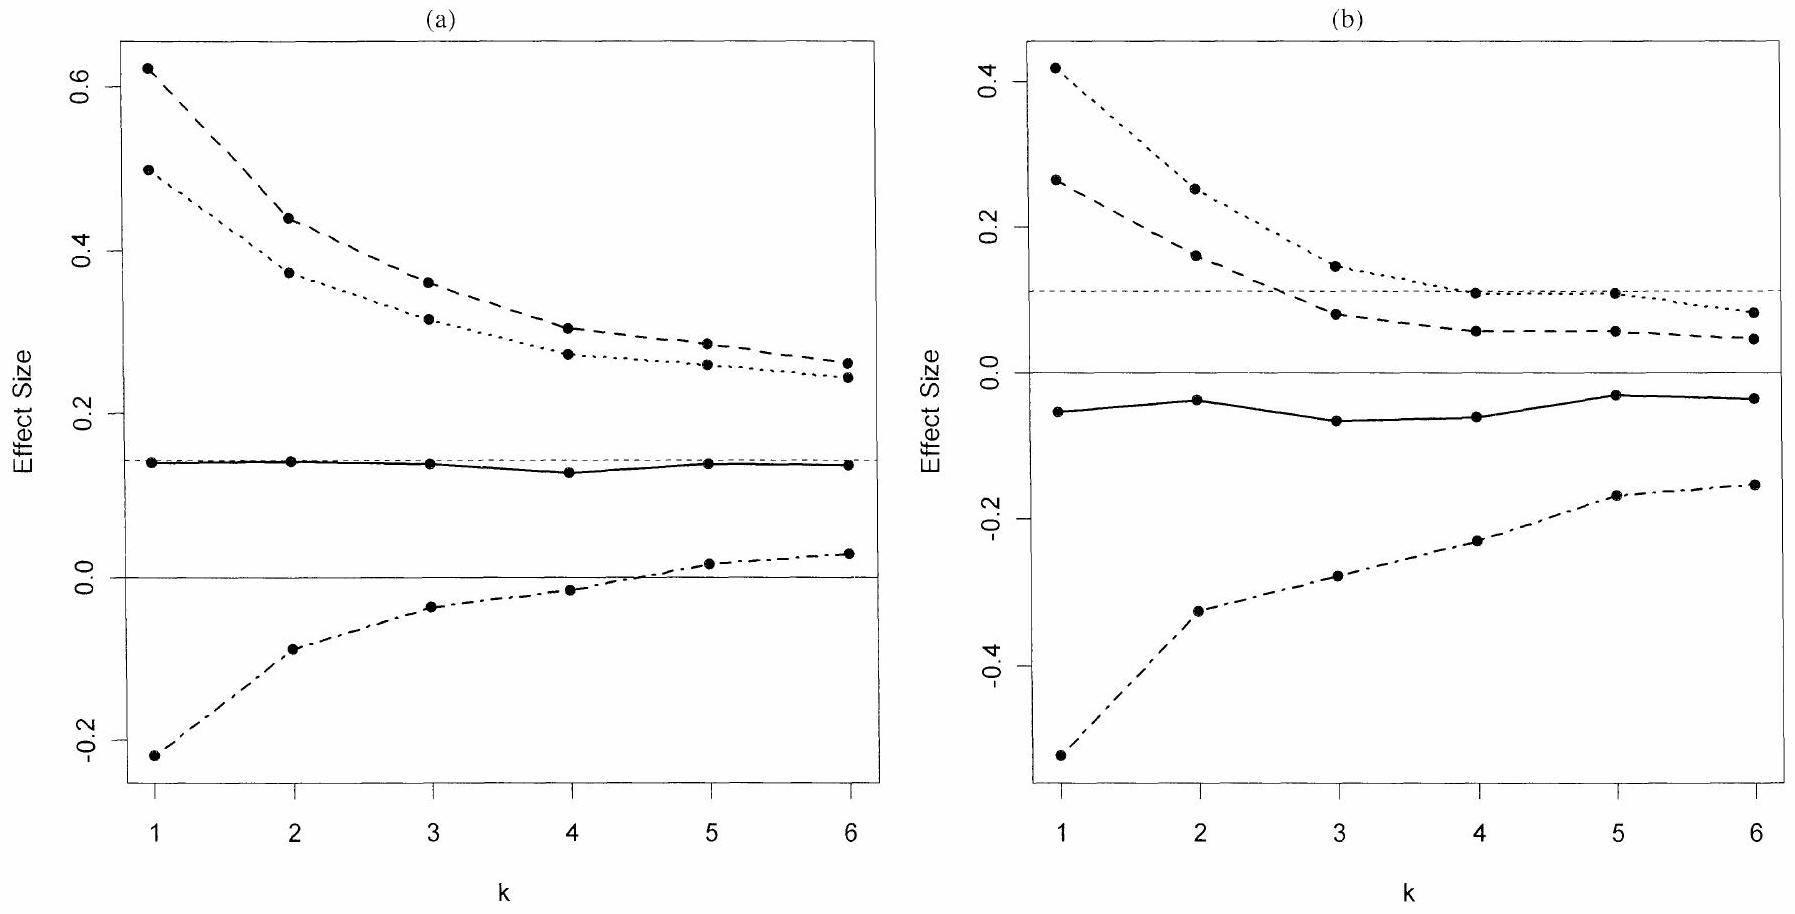
\includegraphics[alt={},max width=\textwidth]{6e684596-3a59-4b5c-b442-c6c146af06f0-10_914_1795_210_198}
\captionsetup{labelformat=empty}
\caption{Figure 1. Sequential monitoring for the primary (a) and secondary (b) endpoints $\left(-, \hat{\Delta}_{i k}^{M e d} ;-\cdots, \hat{\Delta}_{i k}^{F U} ; \cdots \cdots, \hat{\Delta}_{i k}^{U} ; \cdots, \hat{\Delta}_{i k}^{L}\right.$ for $i=1,2$ and $k=1, \ldots, 6$ ).}
\end{center}
\end{figure}

\begin{table}[h]
\begin{center}
\captionsetup{labelformat=empty}
\caption{Table 5. Summary of simulation results}
\begin{tabular}[t]{|l|l|l|l|}
\hline
 & Case 1 & Case 2 & Case 3 \\
\hline
Power for the primary endpoint & . 9842 & . 9842 & . 0252 \\
\hline
Power for the secondary endpoint & . 8941 & . 0210 & . 0033 \\
\hline
Probability of early termination* & . 0069 & . 0069 & . 9059 \\
\hline
Probability of coverage ${ }^{\dagger}$ for $\Delta_{1}$ & . 9669 & . 9630 & . 9717 \\
\hline
Probability of coverage for $\Delta_{2}$ & . 9824 & . 9668 & . 9832 \\
\hline
Expected sample size ${ }^{\ddagger}$ & 725.9 & 671.4 & 636.4 \\
\hline
\end{tabular}
\end{center}
\end{table}

*Early termination occurs when the trial stops for futility before the last analysis.\\
${ }^{\dagger}$ Nominal coverage level is 95\%.\\
${ }^{\ddagger}$ Expected sample size is defined as the mean sample size when the trial stops early or proceeds to the last analysis.

\begin{table}[h]
\begin{center}
\captionsetup{labelformat=empty}
\caption{Table 6. Evaluation of estimators}
\begin{tabular}[t]{|l|l|l|l|}
\hline
 & Median & Unequal weights & Equal weights \\
\hline
\multicolumn{4}{|l|}{Primary endpoint ( $\Delta_{1}=.14238$ )} \\
\hline
Mean & . 14503 & . 1428 & . 1418 \\
\hline
SD & . 03705 & . 04507 & . 05065 \\
\hline
Bias & . 00265 & . 00042 & -. 00056 \\
\hline
MSE ${ }^{1 / 2}$ & . 03714 & . 04507 & . 05065 \\
\hline
\% Bias & . 01859 & . 00298 & -. 00390 \\
\hline
\% MAE* & . 20701 & . 25334 & . 28306 \\
\hline
\multicolumn{4}{|l|}{Secondary endpoint ( $\Delta_{2}=0$ )} \\
\hline
Mean & -. 00314 & . 00004 & -. 00044 \\
\hline
SD & . 03691 & . 04365 & . 05109 \\
\hline
Bias & -. 00314 & . 00004 & -. 00044 \\
\hline
MSE ${ }^{1 / 2}$ & . 03704 & . 04365 & . 05110 \\
\hline
\end{tabular}
\end{center}
\end{table}

\footnotetext{*Percent mean absolute error is defined as mean of absolute bias divided by the effect size.
}
according to the method of Lan and DeMets (1983). The sequential $p$ values also are robust against the underlying homogeneity assumption of treatment effect over time. A significant final sequential $p$ value is interpreted that the underlying null hypothesis has been rejected during the trial, and the type I error rate is controlled at any specified level. Indeed, the latter probabilistic property is true when the final sequential $p$ value is evaluated in long-term hypothetical replications where various deviations would occur. It is in this sense that the proposed $p$ values satisfy the strong repeated sampling principle.

A significant final sequential $p$ value should not automatically lead to any efficacy conclusions, however. This is because the final $p$ value is still significant even when the significance boundary is no longer crossed and extension data reveal that the treatment effect goes in the opposite direction. Additional supportive analyses also are important for examining the treatment effect over time. Various factors can contribute to heterogeneity, including unequal distributions of prognostic factors over time, early patient withdrawals and subsequent treatments, crossover to the experimental treatment by placebo patients after a significance boundary is crossed, and nonproportional hazards in time-to-event analysis. These matters need to be taken into account with sound statistical and clinical judgment, regardless of the group sequential analysis approach taken. Of course, inference is easy when both the final sequential $p$ value and the final repeated $p$ value of Jennison and Turnbull (2000, p. 202) are significant. As an alternative to the final repeated $p$ value, we are currently investigating the final $p$ value proposed by Hall and Ding (2008). We especially recommend this two- $p$ values approach for applications where substantial evidence for efficacy includes a sustained clinical effect after a treatment washout. For example, in studies of drugs for preventing type 2\\
diabetes, the demonstration of a durable delay in the onset of type 2 diabetes after the prevention drug is stopped is necessary to rule out the possibility that the drug only masks diabetes during the treatment period. A group sequential design can be used where a delay in the time to onset of type 2 diabetes can be tested against a significance boundary. Once the boundary is crossed, treatment with the drug stops, and patient follow-up continues for a specified period. A durable delay requires evidence of efficacy at the final analysis, not just when the primary endpoint crosses the boundary at an early time.

Another important property is that standard methods for testing multiple hypotheses can be easily implemented with sequential $p$ values, which expands the number of objectives to be achieved in a group sequential trial. We illustrate this with the motivating example. In the supplemental article we outline test procedures for more applications, where the sequential $p$ values conveniently serve the purpose of controlling multiple type I error rates.

The proposed adaptive design framework permits extension of the trial after a significance boundary is crossed. Similar to existing adaptive designs, the sample size also can be modified. Although the sequential inference procedures satisfy standard error and coverage probabilities criteria, we note that for the latter setting with sample size adjustment, the trial data may not be analyzed efficiently with the proposed inference procedures. Our recommendation is to select the overall sample size and efficacy boundary functions carefully so that for each efficacy endpoint in question, not only is the power adequate, but also the expected time to cross a boundary is minimized. To address issues relating to other efficacy endpoints or safety, the DSMB should rely mainly on extension to future interim analyses while preserving sample size adjustment as a last resort.

We have not touched on the fundamental issue of evaluating statistical evidence. The basic principles of group sequential inference dictate that sample paths reaching the same boundary have identical $p$ values, which, as we show in the supplemental article, is a property shared by existing orderings using maximum likelihood estimates, score statistics, or signed likelihood statistics (Jennison and Turnbull, 2000, p. 180). But should identical $p$ values provide identical evidence against the null hypothesis? In our view, $p$ values provide only the smallest type I error rates at which the null hypothesis can be rejected (Royall 1997, p. 64). As demonstrated in the supplemental article, only the proposed sequential $p$ values can be interpreted as such in the context of a group sequential trial, where various deviations from the original plan can occur in practice. Although the debate about whether $p$ values can validly measure statistical evidence seems to be a matter of recent history (Armitage 1975, sec. 2.5; Dupont 1983; O'Hagan 1989), various logical difficulties with emerging adaptive designs using combination tests are reinvigorating this debate, which once again calls for an evidentiary approach to statistical inference (Frisen 2006).\\[0pt]
[Received January 2007. Revised July 2008.]

\section*{REFERENCES}
Armitage, P. (1975), Sequential Medical Trials (2nd ed.), New York: Wiley.\\
Canner. P. L. (1983), "Monitoring of the Data for Evidence of Adverse or Beneficial Treatment Effects." Controlled Clinical Trials, 4, 467-483.\\
CHMP (2007). "On Methodological Issues in Confirmatory Clinical Trials Planned With an Adaptive Design," CHMP/EWP/2459/02.\\
Cox, D. R., and Hinkley, D. V. (1974), Theoretical Statistics, London: Chapman \& Hall.\\
Cui, L., Hung, H. M. J., and Wang, S. J. (1999), "Modification of Sample Size in Group Sequential Clinical Trials." Biometrics, 55, 853-857.\\
DeMets, D. L. (1984), "Stopping Guidelines vs. Stopping Rules: A Practitioner's Point of View." Communications in Statistics, Part A-Theory and Methods, 13, 2395-2418.\\
DeMets, D. L., and Ware, J. H. (1980), "Group Sequential Methods for Clinical Trials With a One-Sided Hypothesis," Biometrika, 67, 651-660.

\begin{itemize}
  \item (1982), "Asymmetric Group Sequential Boundaries for Monitoring Clinical Trials." Biometrika, 69, 661-663.\\
Dupont, W. D. (1983), "Sequential Stopping Rules and Sequential Adjusted $p$ Values: Does One Require the Other?" (with discussion), Controlled Clinical Trials, 4, 3-35.\\
Ellenberg, S. S., Fleming. T. R., and DeMets, D. L. (2002), Data Monitoring Committees in Clinical Trials: A Practical Perspective. West Sussex, U.K.: Wiley.\\
Fisher, L. (1998), "Self-Designing Clinical Trials," Statistics in Medicine, 17, 1551-1562.\\
Frisen, M. (2006), Discussion of "Are Flexible Designs Sound?" by Burnman, C. F., and Sonesson, C., Biometrics, 62, 678-680.\\
Hacking, I. (1965), Logic of Statistical Inference, Cambridge, U.K.: Cambridge University Press.\\
Hall, W. J., and Ding, K. (2008), "Sequential Tests and Estimates After Overrunning Based on $p$-Value Combination," IMS Collections, Pushing The Limits of Contemporary Statistics: Contributions in Honour of Jayanta K. Ghosh, 3. 33-45.\\
Hall. W. J., and Liu, A. (2002), "Sequential Tests and Estimators After Overrunning Based on Maximum-Likelihood Ordering," Biometrika, 89, 699-707.\\
ICH (1998), "Guidance on Statistical Principles for Clinical Trials," Federal Register, 63, 49583-49598.\\
Jennison, C., and Turnbull. B. W. (1989), "Interim Analysis: The Repeated Confidence Interval Approach" (with discussion), Journal of the Royal Statistical Society, Ser. B, 51, 305-361.\\
(2000), Group Sequential Methods With Applications to Clinical Trials, Boca Raton, FL: Chapman \& Hall.\\
Lan, K. K. G., and DeMets, D. L. (1983), "Discrete Sequential Boundaries for Clinical Trials," Biometrika, 70, 659-663.\\
Lan, K. K. G., and Wittes, J. (1994), "Data Monitoring in Complex Clinical Trials: Which Treatment Is Better?" Journal of Statistical Planning and Inference. 42. 241-255.\\
Lan, K. K. G., Lachin, J. M., and Bautista, O. (2003), "Over-Ruling a Group Sequential Boundary: A Stopping Rule vs. a Guideline," Statistics in Medicine. 22, 3347-3355.\\
Liu, Q., and Anderson, K. M. (2008), "Theory of Inference for Adaptively Extended Group Sequential Designs With Applications in Clinical Trials," available at \href{http://www.amstat.org/publications/jasa/supplemental_materials}{http://www.amstat.org/publications/jasa/supplemental\_materials}.\\
Liu, Q., and Pledger, G. W. (2006), "On Design and Inference for Two-Stage Adaptive Clinical Trials With Dependent Data," Journal of Statistical Planning and Inference, 136, 1962-1984.\\
Liu, Q., Proschan, M. A., and Pledger, G. W. (2002), "A Unified Theory of TwoStage Adaptive Designs," Journal of the American Statistical Association, 97. 1034-1041.\\
O'Hagan, A. (1989), Discussion of "Interim Analyses: The Repeated Confidence Interval Approach," by C. Jennison and B. W. Turnbull, Journal of the Royal Statistical Society. Ser. B, 51. 342.\\
Proschan, M. A. (1999), "Properties of Spending Function Boundaries." Biometrika, 86, 466-473.\\
Proschan, M. A., Lan, K. K. G., and Wittes, J. T. (2006), Statistical Monitoring of Clinical Trials, New York: Springer.\\
Royall, R. (1997), Statistical Evidence: A Likelihood Paradigm, London: Chapman \& Hall.\\
Whitehead, J. (1992), "Overrunning and Underrunning in Sequential Clinical Trials," Controlled Clinical Trials, 13, 106-121.\\
(1999), "On Being the Statistician on a Data and Safety Monitoring Board." Statistics in Medicine, 18, 3425-3434.
\end{itemize}

\end{document}
